\documentclass[10pt,a4paper]{article}
\usepackage[margin=1in]{geometry}

\usepackage[T1]{fontenc}
\usepackage{amssymb}
\usepackage{amsthm}
\usepackage{physics}
\usepackage[dvipsnames]{xcolor} %colors
\usepackage{float} % <- importante
\usepackage[draft,inline,nomargin]{fixme} \fxsetup{theme=color} % Comments
\definecolor{jacolor}{RGB}{200,40,0}
\FXRegisterAuthor{ja}{aja}{\color{jacolor}JA}
\FXRegisterAuthor{sn}{asa}{\color{OliveGreen}Saul}

\usepackage[inline]{showlabels}
\renewcommand{\showlabelfont}{\scriptsize\color{gray!75}}
\renewcommand{\showlabelrefline}{\hrule width 0pt height -1.8ex depth 0pt}

\usepackage[spanish]{todonotes}
%\setuptodonotes{inline,color=blue!25,tickmarkheight=25mm,size=\small}
\setuptodonotes{
  inline,
%  color=orange!25,           % Background color
  backgroundcolor=red!30, % Same as color (alternative name)
  size=\small,            % \tiny, \scriptsize, \footnotesize, \small, \normalsize, etc.
  tickmarkheight=10mm,     % Height of margin marker
}

\usepackage{hyperref}
\hypersetup{
colorlinks=true,
linkcolor=blue,
filecolor=blue,      
citecolor=blue,
urlcolor=blue,
pdftitle={},
pdfauthor=author={},
}

\usepackage[
backend=bibtex,
style=phys,
maxbibnames=5,
biblabel=brackets,
hyperref=true,
arxiv=abs,
eprint=true,
url=false,
doi=false
]{biblatex}
\AtEveryBibitem{\clearfield{note}}
\AtEveryBibitem{\clearfield{pubstate}}  % Remove pubstate from all entries
\addbibresource{symmetries_and_chaos.bib} 
\graphicspath{{img/}}
\newcommand{\eref}[1]{eq.~(\ref{#1})} 
\newcommand{\sref}[1]{sec.~\ref{#1}}
%\newcommand{\tref}[1]{table~\ref{#1}}
\newcommand{\Eref}[1]{Eq.~(\ref{#1})} 
\newcommand{\Sref}[1]{Sec.~\ref{#1}}
\newcommand{\Appref}[1]{Appendix~\ref{#1}}
\newcommand{\Fref}[1]{Fig.~\ref{#1}}  
\newcommand{\Tref}[1]{Table~\ref{#1}}

\title{Notas}
%}}}
\begin{document}
\section{Bose Hubbard Model for bosons:}
 \begin{equation}
            \hat{H}
            = -\frac{J}{2} \sum_{\langle i,j\rangle} \!\left(\hat{a}_i^{\dagger}\hat{a}_j + \hat{a}_j^{\dagger}\hat{a}_i\right)
            + \frac{U}{2}\sum_{i}\hat{n}_i(\hat{n}_i - 1).
            \end{equation}
        $\hat{a}_i^{\dagger}, \hat{a}_j$ are ladder operators and $\hat{n}_i=\hat{a}_i^{\dagger}\hat{a}_i$, J and U are related to the kinetics and interactions among the bosons, respectively.
    \section{Mean Spacings Ratio}
The following generalization was used:
    \begin{equation}
      r^{k}_n=\frac{\min(s^{k}_n,s^{k}_{n-1})}{\max(s^{k}_n,s^{k}_{n-1})}.
      \end{equation}
Employing only a first order corrleation yields a characteristic value of $\ev{r}_{GOE}=0.5307$
     and $\ev{r}_{Poisson}=0.38629$.
Employing several BH realizations, with different J/U values, a region of values was found to be in accordance, at least for fist order correlations, with the GOE.
\begin{figure}[H]
\centering
\includegraphics[width=1\textwidth]{Map.pdf}
\caption{Mean spacing ratio of first correlation of several BHH hamiltonians with differnt $J/U$ values. Notice that from 0.5 to 10, the mean value is similar to the GOE prediction. Using a BHH of 9 sites and 9 bosons. }
\label{fig:Map}
\end{figure}
\textit{The following figures show the behavior of $\ev{r^{k}_n}$ for all k values ranging from k=1 to k=Total amount of eigenvalues of several BH realizations using differnt J/U. the Poisson and GOE characteristic curves are given as reference.}

\textbf{Considering only J/U values located in the chaos region:}
\begin{figure}[H]
\centering
\includegraphics[width=1.1\textwidth]{BHMeanKChaosRegionLowK.pdf}
\caption{Mean spacing ratio for low k of several BHH hamiltonians of dim 8,8 with different $J/U$ values located in the chaos regime. }
\label{fig:BHMeanKChaosRegionLowK}
\end{figure}
\begin{figure}[H]
    \centering
    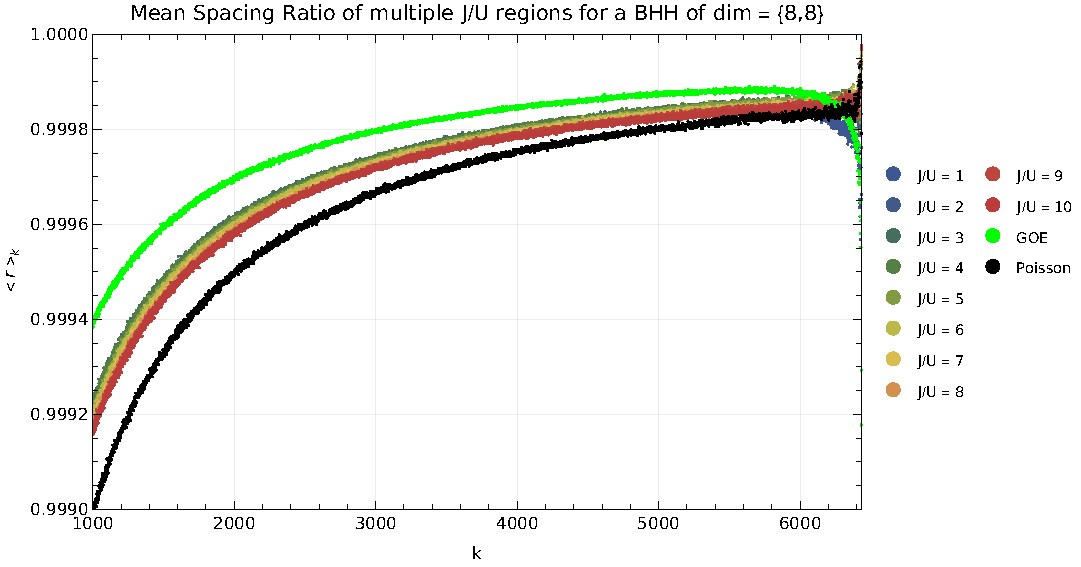
\includegraphics[width=1.1\textwidth]{BHMeanKChaosRegionMiddleK.pdf}
    \caption{Mean spacing ratio as k grows of several BHH hamiltonians of dim 8,8 with different $J/U$ values located in the chaos regime. }
    \label{fig:BHMeanKChaosRegionMiddleK}
\end{figure}
\textbf{Considering low J/U values located in the transition phase between chaos and integrability:}
\begin{figure}[H]
\centering
\includegraphics[width=1.1\textwidth]{BHMeanKNearChaosAndPoissonRegionLowK.pdf}
\caption{Mean spacing ratio for low k of several BHH hamiltonians of dim 8,8 with different $J/U$ values located in transition phase.}
\label{fig:BHMeanKNearChaosAndPoissonRegionLowK}
\end{figure}

\section{Spectral form factor (SFF)}
The SFF can be decomposed into the following sums:
\begin{align}
\label{eq:sff}
K(t) &= \frac{1}{N^2} \overline{\sum_{k,l} e^{-i (E_k - E_l) t}} \\
&= 
1
+ \frac{2}{N^2}\Re\Bigg[
\overline{
\sum_{k=1}^{N-1}
e^{-i (E_{k+1} E_k) t} 
} +
\overline{
\sum_{k=1}^{N-2}
e^{-i (E_{k+2} - E_k) t} 
}
+ \ldots +
\overline{
e^{-i (E_N - E_1) t} 
}
\Bigg].
\label{eq:sff:spacings}
\end{align}
\begin{figure}[H]
    \centering
    \includegraphics[width=0.9\textwidth]{CompSectAndTime.pdf}
    \caption{Comparison between using just time averanging and time averanging with sector averanging (red line is the GOE prediction).}
    \label{fig:CompSectAndTime}
\end{figure}

\section{Bose Hubbard and SFF}
Two Bose Hubbard configurations where tested, one with periodic boundary conditions and the other with open boundary conditions.
For both configurations, multiple J/U realizations where made.

\textit{For the moment, a stricking difference is noted in the scaling among both configurations.}
\begin{figure}[H]
    \centering
    \includegraphics[width=1.1\textwidth]{SFFBHPeriodicAndOpen.pdf}
    \caption{SFF of both configurations, periodic and open boundary conditions, for multiple J/U realizations. }
    \label{fig:SFFPeriodicOpen}
\end{figure}
It is to be noted that, considering periodic boundary conditions, the J/U values that are regarded as chaos in the open frontier conditions, are not in general in accordance with what is seen with the SFF results for periodic conditions. 
In particular, the following figure shows that some J/U values are linked with integrability behavior.
\begin{figure}[H]
    \centering
    \includegraphics[width=1.1\textwidth]{SFFBHPeriodic1.pdf}
    \caption{SFF of periodic boundary conditions, for multiple J/U realizations. }
    \label{fig:SFFPeriodic}
\end{figure}
\end{document}
